\section{Aufbau}
\label{sec:Aufbau}

Der Versuchsaufbau für den ersten Teilversuch ist in Abbildung \ref{fig:Aufbau1} zu sehen. Der Referenz-Ausgang erzeugt die Signalspannung $U_.{sig}$ und der Oszillator-Ausgang erzeugt die Referenzspannung $U_.{ref}$. Die Frequenzen beider Spannungen sind identisch, die Amplitude von $U_.{sig}$ ist verstellbar. Die Signalspannung ist über einen Rauschgenerator und einen Vorverstärker mit einem Bandpassfilter verbunden. Im Detektor wird das Ausgangssignal nach dem Bandpassfilter mit der Referenzspannung gemischt und über einen Tiefpass-Verstärker am Oszilloskop angezeigt. Dabei kann vor dem Detektor über den Phasenschieber die Phase des Referenzsignals eingestellt werden.

\begin{figure}
	\centering
	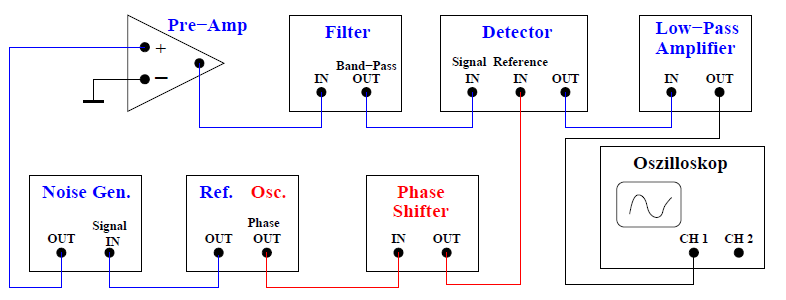
\includegraphics[width=\linewidth-40pt,height=\textheight-40pt,keepaspectratio]{content/images/Aufbau1.png}
	\caption{Der Versuchsaufbau für den ersten Teilversuch\cite{V303}}
	\label{fig:Aufbau1}
\end{figure}

\noindent Der zweite Versuchsaufbau (Abbildung \ref{fig:Aufbau2}) ist dem ersten ähnlich, nur das hier anstatt des Rauschgenerators ein Photodetektor verwendet wird, der das ausgesendete Licht einer periodisch blinkenden Leuchtdiode in elektrische Signale umwandelt.

\begin{figure}
	\centering
	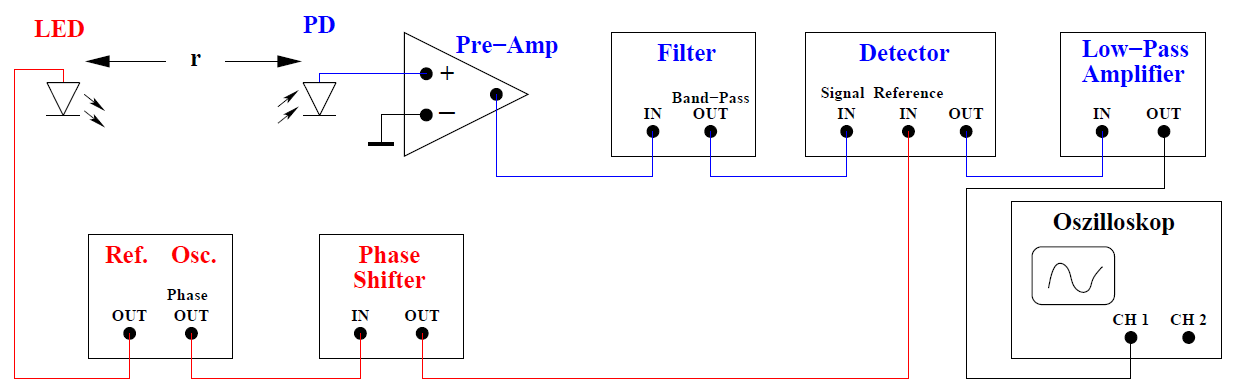
\includegraphics[width=\linewidth,height=\textheight,keepaspectratio]{content/images/Aufbau2.png}
	\caption{Der Versuchsaufbau für den zweiten Teilversuch\cite{V303}}
	\label{fig:Aufbau2}
\end{figure}